	
\documentclass[12pt,a5paper]{article}

\usepackage[T1]{fontenc} % font encoding, lubab õ tähte kasutada
\usepackage[utf8]{inputenc} % oleme siiski 21. sajandis, vajadusel on ka olemas utf8x
\usepackage{lmodern} % lmodern ja micrtype käivad käsikäes, teeb teksti ilusamaks
\usepackage{tikz}
\usetikzlibrary{decorations.pathreplacing, positioning}
\usepackage{microtype}
\usepackage[estonian]{babel} % eesti keele poolitamisreeglid jpm
\usepackage[per = fraction, expproduct=cdot, decimalsymbol=comma]{siunitx} % http://www.bakoma-tex.com/doc/latex/siunitx/siunitx.pdf
\usepackage{graphicx} 
\usepackage{wrapfig}
\usepackage{epstopdf} %minul on vaja, et .eps pilte saada
\usepackage{icomma} %koma arvust mõistlikul kaugusel
\usepackage{amsmath}
\usepackage{caption}
\usepackage{pgfplots}
\usepackage{float}
\usepackage{enumerate} %loendite tegemiseks
\usepackage{subcaption}

\special{papersize=14.85cm,21cm}

%paneme kõik mõõdud paika
\topmargin=-2.5cm \textheight=18.5cm \textwidth=12.77cm
\oddsidemargin=-1.5cm  \evensidemargin=-1.5cm
\setlength{\parindent}{0pt} \setlength{\parskip}{6pt} \sloppy

\relpenalty=10000 \binoppenalty=10000 % Tekstisisestes valemites reavahetusi ärgu olgu


\pagestyle{empty} % ilma leheküljenumbrita

\newcommand{\numb}[1]{\vspace{5pt}\textbf{\large #1}}
\newcommand{\nimi}[1]{(\textsl{\small #1})}
\newcommand{\punktid}[1]{(\emph{#1~p.})}
\newcounter{ylesanne}
\newcommand{\yl}[1]{\addtocounter{ylesanne}{1}\numb{\theylesanne.} \nimi{#1} \newblock{}}
\newcommand{\pp}[1]{[\textbf{#1~p.}]}
\newcommand{\pv}[1]{\quad \hbox{[\textbf{#1~p.}]}}
\newcommand{\ue}[1]{\underline{\emph{#1}}}
\newcommand{\hence}{\quad \Rightarrow \quad}
\newcommand{\autor}[1]{\emph{ Autor: #1.\\}}
\newcommand{\lautor}[1]{\emph{ Lahenduse autor: #1.\\}}


\begin{document}

\begin{center}
\textbf{\Large Eesti koolinoorte 66. füüsikaolümpiaad} \vspace{2pt}

\emph{06. aprill 2019. a. Vabariiklik voor.}

\emph{{\bf Gümnaasiumi} ülesannete lahendused}


\end{center}


\yl{AUTOD} \punktid{6} Kuna autod jäävad seisma samaaegselt, siis läheme ühe ühe autoga seotud taustsüsteemi.
Autode suhteline kiirus üksteise suhtes on $v = v_1+v_2 = \SI{180}{km/h}=\SI{50}{m/s}$\\
Autode pidurdusteekond on kokku $2=\SI{600}{m}$ ning lõppkiirus on $\SI{0}{m/s}$, siis pidurdamiseks kulunud aeg on
\[ s = \frac{v + v_0}{2}\cdot t \quad\quad\Rightarrow\quad\quad t = \frac{2s}{v+v_0} = \SI{24}{s} \]

\yl{SAUNAUKS} \punktid{8} Saunakerisele visatud vee aurustamine lisas saunaruumi rõhu: 

\[ p = {\rho V_v  \over \mu} \cdot {RT\over V} = {200 \over 18} \cdot {8,\!314 \cdot 373 \over 3\cdot2,\!5\cdot2,\!4} \approx \SI{1914}{Pa}. \] 

kus me kasutasime teadmist, et auru temperatuur $T=\SI{373}{K}$. Saunaukse pindala $S_u = 0,\!7 \cdot 1,\!9 = \SI{1,33}{m^2}$ ning talle mõjub jõud $F = p S_u \approx \SI{2546}{N}$.
Selleks, et leili rõhk ust lahti ei teeks, peab ukse hingedele mõjuv hõõrdejõu moment olema vähemalt:

\[ \tau = { F l } = { 2546 \cdot {0,\!7 \over 2 } } \approx \SI{891}{N/m}.\]

\newpage

\begin{wrapfigure}{r}{0.41\textwidth}
  \vspace{-15pt}
  \begin{center}
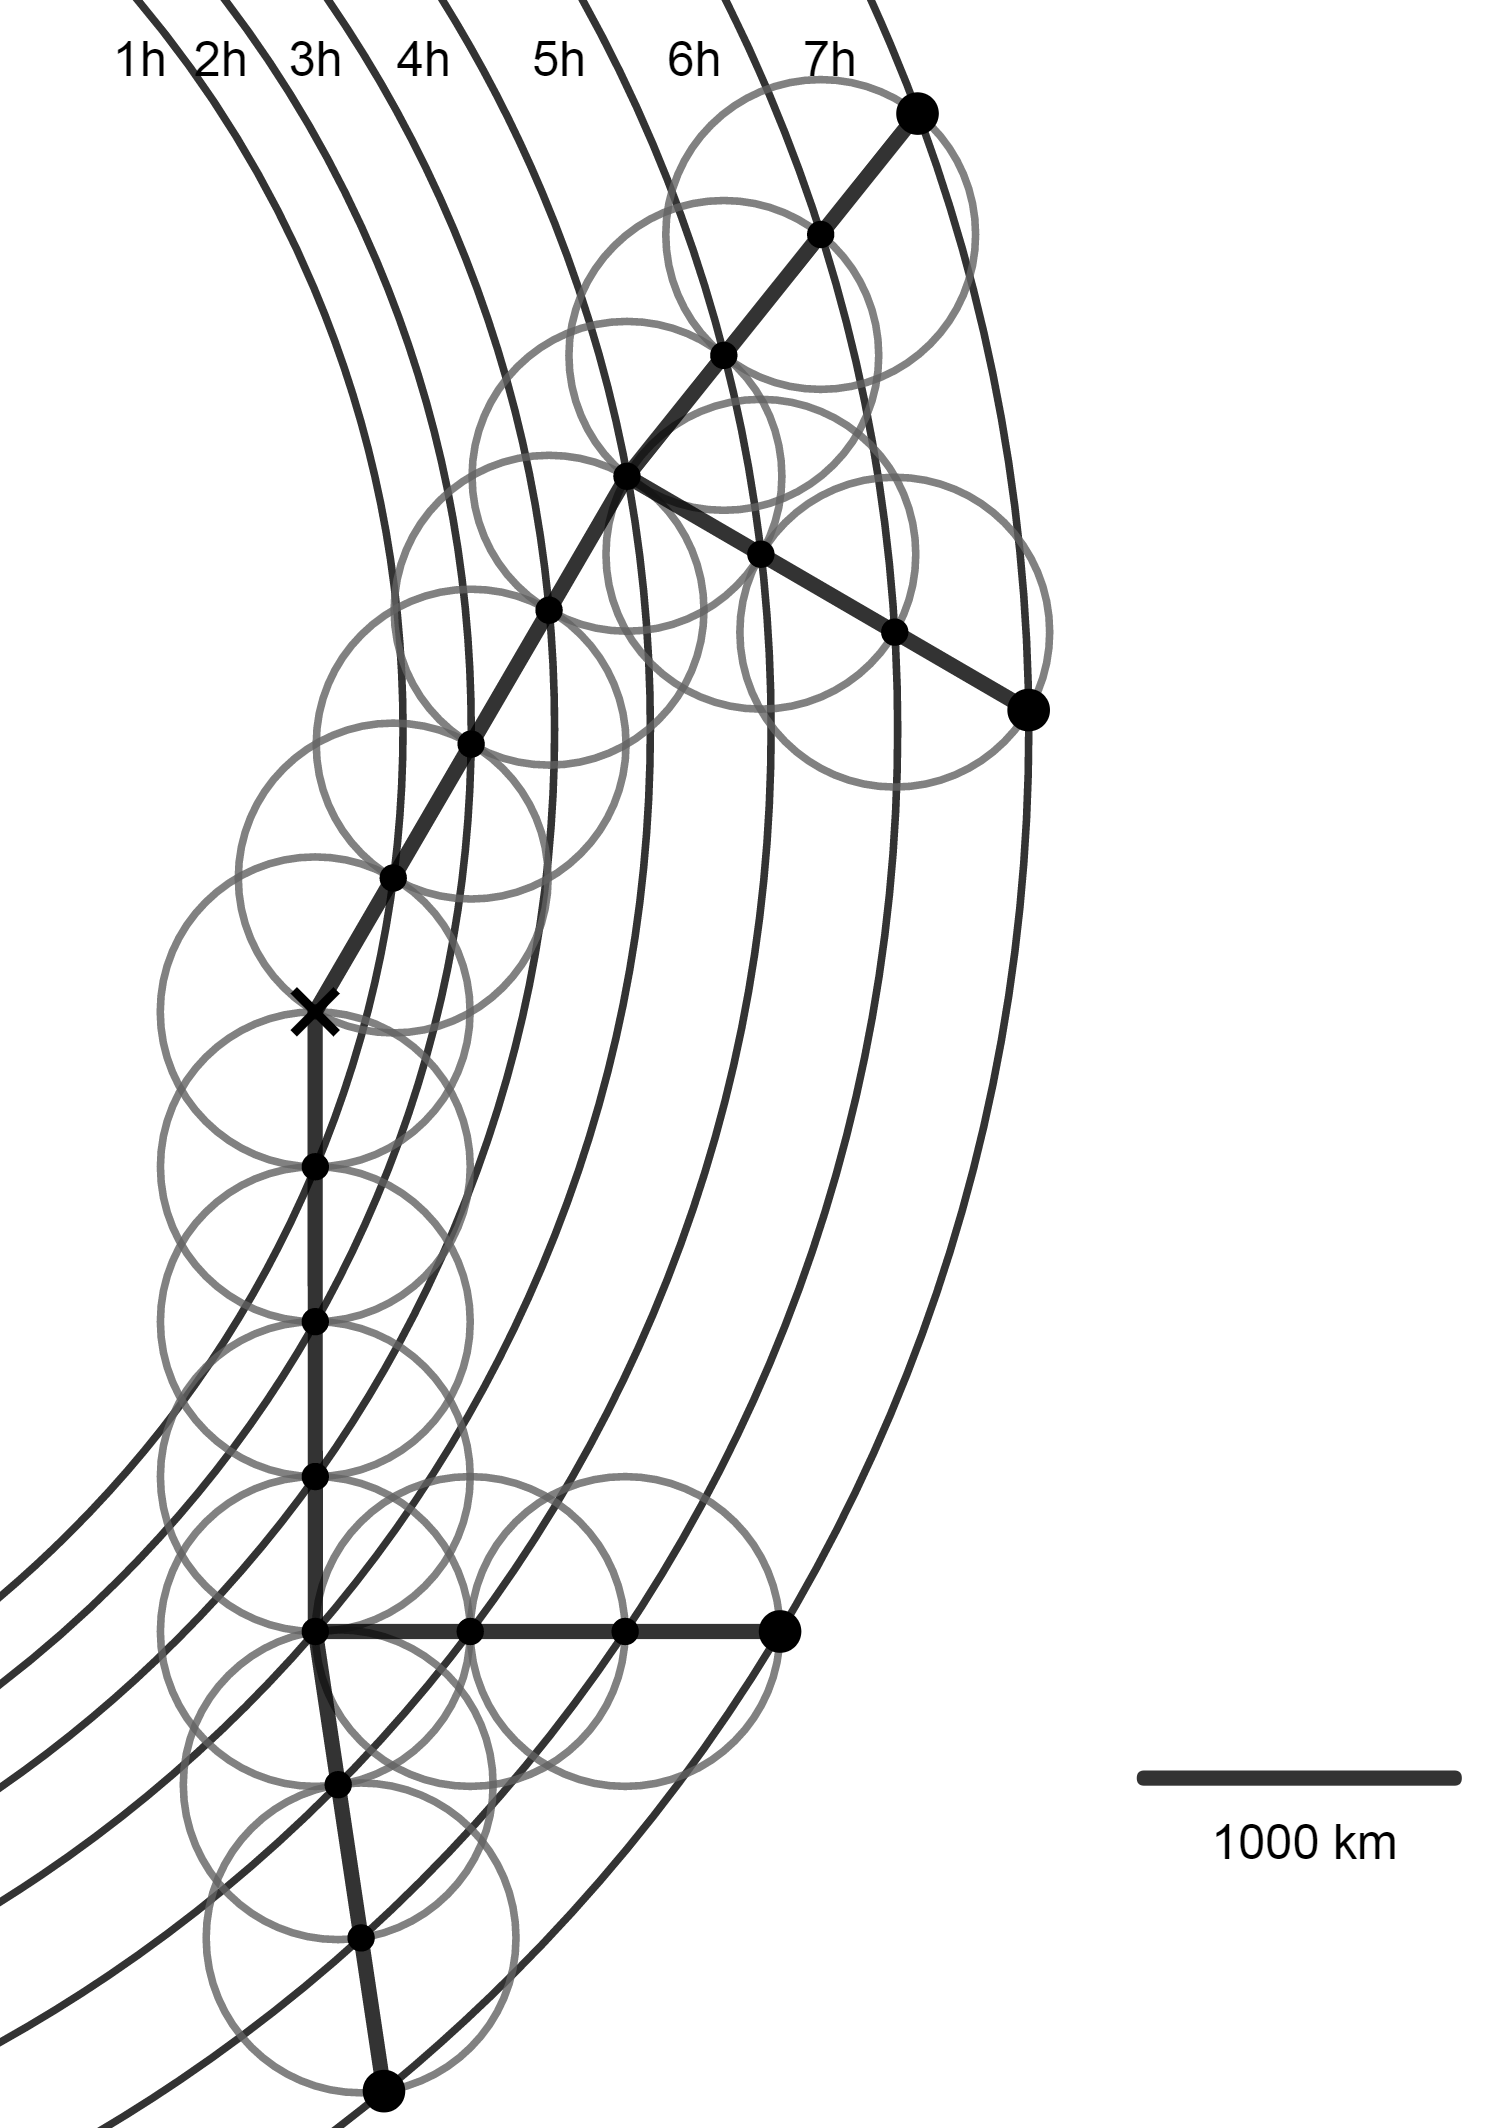
\includegraphics[scale=0.15]{LennukSolutionG.png}
    % Pildi allikas Wikimedia Commons https://upload.wikimedia.org/wikipedia/commons/4/4f/Curling_stones.jpg
  \end{center}
  \vspace{-20pt}
\end{wrapfigure}

\yl{LENNUK} \punktid{8} Teame, et suured ringjooned märgivad lennuki asukohta iga tunni järel ning ühe tunniga läbib lennuk $\SI{500}{km}$. Joonisel oleva mõõtkava järgi saame $\SI{500}{km}$ vastava pikkuse joonisel. Võtame selle pikkuse ja joonestame sirkliga vastava raadiusega ringjoone lennuki algasukoha ümber. See ringjoon märgib lennuki asukohta $1h$ pärast õhkutõsu ning selle lõikepunktid olemasoleva esimese suure ringjoonega (mis märgib samuti lennuki asukohta $\SI{1}{h}$ pärast õhkutõsu) annavad meile lennuki võimalikud asukohad $\SI{1}{h}$ pärast. Kuna me ei tea, millises suunas lennuk lendas, peame lennuki teekonda mõlemast punktist edasi konstrueerima, joonestades uute punktide ümber samuti $\SI{500}{km}$ vastava ringjoone. Kuna aga teame, et lennuk lendas $\SI{4}{h}$ järjest otse, saame hakata lõikepunkte välistama, sest sobivad punktid moodustavad sirge. $\SI{4}{h}$ vastava ringjoone juures teame vaid seda, et lennuk muutis suunda. Seega saame kummagi algse teekonna kohta veel 2 võimalikku uut suunda (kokku 4 võimalikku suunda). Teades, et lennuk lendas edaspidi samuti vaid otse, saame kõik 4 teekonda lõpuni konstrueerida.

\yl{KONVEIER} \punktid{8} Olles täielikult esimesel lindil, on plaadi kiirus $v_1$ ning teisel lindil $v_2$. Plaadi kiirus muutub üleminekukohas $v_1$-lt $v_2$-le, kui hõõrdejõud teise konveierilindiga ületab hõõrdejõu esimese konveierilindiga. Olgu plaadi mass $M$ ning plaadi joontihedus piki konveierit $\rho = M/l$. Piirjuhul saame hõõrdejõudude võrdsusest:
$$\mu_{1}M_1g = \mu_{2}M_2g$$
kus $M_1$ ja $M_2$ on vastavalt esimese ja teise lindi peal oleva plaadi osa massid. Olgu esimesel lindil oleva osa pikkus $l_1$ ning teisel osal $l_2$. Kasutades joontihedust saame:
$$\mu_{1} \rho l_1 g = \mu_{2}\rho l_2 g$$.
Taandades ühised kordajad saame võrrandisüsteemi:
$$\mu_{1} l_1 = \mu_{2} l_2$$
$$l_1 + l_2 = l$$
Siit saame avaldada $l_1$-e:
$$l_1 = \frac{l}{1+\frac{\mu_{1}}{\mu_{2}}}$$

\begin{center}
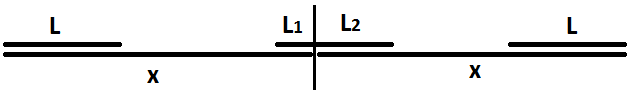
\includegraphics[scale=0.5]{Konveier.png}
\end{center}


Joonisel on kujutatud plaadi algasend, lõppasend ning piirjuht, kus kiirus muutub (tühiselt väikese aja jooksul). Algasendist piirjuhuni läbib plaat vahemaa $x - l_1$ kiirusel $v_1$. Piirjuhust lõppasendini läbib plaat vahemaa $x - l_2$ kiirusel $v_2$. Seega koguaeg:
$$t = \frac{x - l_1}{v_1} + \frac{x - l_2}{v_2}$$
Asendades saame:
$$t=\frac{v_2 x - v_2 l_1 + v_1 x - v_1 l_2}{v_1 v_2} =$$
$$\frac{x(v_1 + v_2) - lv_1 - l_1 v_2 + l_1 v_1}{v_1 v_2} =$$
$$\frac{x(v_1 + v_2) - lv_1 + \frac{l(v_1 - v_2)}{1+\frac{\mu_{1}}{\mu_{2}}}}{v_1 v_2}$$



\yl{JÄÄKEEGEL} \punktid{10} Esmalt veendume selles, et esialgu liikuva kivi märklaua keskele jõudmiseks peab kivide vahel toimuma tsentraalne otsepõrge. Oletame vastuväiteliselt, et liikuva kivi trajektoori pikendus ei läbi enne põrget seisva kivi massikeset, vaid möödub sellest näiteks paremalt poolt (liikumise sihis vaadatuna). Kuna kivide ristlõiked on ringikujulised ja eeldame, et kivi massikese asub ringi keskel, siis mõjuvad kivide vahel põrke ajal jõud piki nende massikeskmeid ühendavat sirget. Jagades liikumatu kivi poolt liikuvale kivile avaldatava jõu kaheks komponendiks, millest üks on piki kivi esialgset trajektoori ja teine sellega risti, näeme et jõu ristikomponent on suunatud liikumise sihist paremale. Seega pöördub liikuva kivi trajektoor põrke tulemusel veel rohkem paremale ja ei saa läbida märklaua keskpunkti. Järelikult peab ülesande tingimuste täitmiseks toimuma tsentraalne otsepõrge ja saame järgnevalt olukorda vaadelda ühemõõtmelisena.

Märklaua keskele jõudmiseks peab esialgu liikuv kivi pärast põrget teatud kiirusega edasi liikuma ja seejärel jääga hõõrdumise tõttu seisma jääma. Tähistame kiirused: $v_0$ ja $v$ -- esialgu liikuva kivi kiirus enne ja pärast põrget ning $u$ -- esialgu seisva kivi kiirus pärast põrget. Impulsi jäävuse seadusest:
\begin{equation}
mv_0 = mv + mu,
\end{equation}
kus $m$ on kivi mass, mis nagu näha välja taandub. Samuti saame kirjutada energia jäävuse seaduse
\begin{equation}
\left(1-\eta\right)\frac{mv_0^2}{2} = \frac{mv^2}{2} + \frac{mu^2}{2},
\end{equation}
kus $\eta = \num{0.4}$ on põrkel kaduma läinud energia osakaal.

Kiiruse $v$ jaoks kehtib tingimus
\begin{equation}
\frac{mv^2}{2} = \mu mgs,
\end{equation}
ehk esialgu liikuva kivi kineetiline energia pärast põrget on võrdne hõõrdejõu tööga kivi seismajäämisel. Põrke hetkel on esialgu liikuva kivi keskkoha kaugus märklauast võrdne kivi läbimõõduga ehk $s = D$ ja $v = \sqrt{2\mu gD}$.

Kiiruse $v_0$ leidmiseks avaldame impulsi jäävuse seadusest $u = v_0 - v$ ja asetame selle energia jäävuse avaldisse:
\begin{equation}
\left( 1 - \eta \right)v_0^2 = v^2 + \left(v_0 - v\right)^2, 
\end{equation}
millest
\begin{equation}
\eta v_0^2 - 2v_0 v + 2v^2 = 0.
\end{equation}
Saadud ruutvõrrandi lahend on
\begin{equation}
v_0 =  \frac{v\left( 1 \pm \sqrt{1-2\eta} \right)}{\eta}
\end{equation}
ehk kasutades eelnevalt leitud $v$ avaldist, saame
\begin{equation}
v_0 =  \frac{\sqrt{2\mu gD}\left( 1 \pm \sqrt{1-2\eta} \right)}{\eta}.
\end{equation}
Vastavalt märgile ruutvõrrandi lahendi valemis saaksime kiirusteks

\begin{center}
\begin{tabular}{|c|c|c|}
\hline 
 & $+$ & $-$ \\ 
\hline 
$v_0$ & \SI{1.22}{m/s} & \SI{0.47}{m/s} \\ 
\hline 
$v$ & \SI{0.34}{m/s} & \SI{0.34}{m/s} \\ 
\hline 
$u$ & \SI{0.88}{m/s} & \SI{0.13}{m/s} \\ 
\hline 
\end{tabular}
\end{center}

Kuna kivid ei saa pärast põrget üksteisest läbi minna, siis peab kehtima $u > v$ ja füüsikaliselt sobib ainult pluss-märgiga lahend ehk kivi kiirus enne põrget on $v_0 = \SI{1.2}{m/s}$.

\begin{wrapfigure}[7]{r}{0.41\textwidth}
  \vspace{-25pt}
  \begin{center}
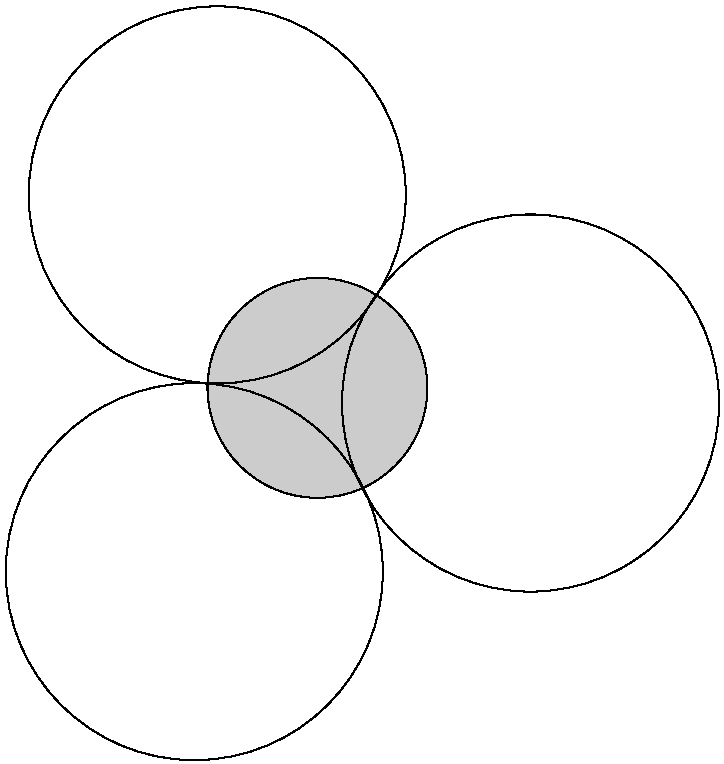
\includegraphics[scale=0.3]{l6ks-lah.pdf}
    % Pildi allikas Wikimedia Commons https://upload.wikimedia.org/wikipedia/commons/4/4f/Curling_stones.jpg
  \end{center}
  \vspace{-20pt}
\end{wrapfigure}

\yl{LÕKS} \punktid{10} Kuulikese trajektoor silindris koosneb kolmest kaarejupist nii nagu näidatud joonisel. Nagu jooniselt näha, igale kaarejupile vastav kesknurk on 60 kraadi, seega trajektooride kesknurkade summa on pool täisringist, st kuulike veedab silindris pool tsüklotronperioodist  $t=T/2=\pi\frac m{qB}$.





\yl{3 RUUTU} \punktid{10} Lihtsustame skeemi arvestades sellega, et ideaalsete ampermeetrite sisetakistus on null: me võime lühistada need sõlmpunktid, mis on ühendatud juhtmega läbi ampermeetri. Selleks, et olla kindel vigadeta skeemi teisendamises tähistame takistid numbritega ja sõlmpunktid tähtedega, vt esimene joonis. Paneme tähele, et Kirchoffi vooluseaduse tõttu näitavad ampermeetrid vastavalt esimese ja viienda, seitsmenda ja neljanda ning kaheksanda ja neljanda  takisti voolude vahet.

Seejärel alustame sõlmpunktide märkimisest ja ühendame need samade takistitega, mis algseski skeemis, tulemus on näidatud teisel joonisel. Viimase sammuna  jagame sõlmpunkti C kaheks osaks lõigates mõtteliselt läbi joonise sümmeetriateljel oleva vertikaalse juhtme; seda võib teha,  sest sümmeetria tõttu puudub selles vertikaalses juhtmes vool. Nüüd on juba lihtne leida takistite voolud: takistitest 8 ja 9 koosneva ahela kogutakistus on $r_8=\SI {6}\ohm$, seetõttu  läbib neid vool $i_8=\mathcal E/r_8=\SI 8A$. Punktide B ja D vahelise viiest takistist koosneva ahelajupi takistus on $\frac 67\SI {}\ohm$ ning seega ülemise ahelapoole kogutakistus on $r_1=\frac {48}7\SI {}\ohm$ ja takisti 1 vool $i_1=\mathcal E/r_1=\SI 7A$. Seega langeb takistite 1 ja 7 peale kokku pinge $2i_1R=\SI {42}V$, mistõttu sõlmede B ja D vaheline pinge on $V_5=\mathcal E-2i_1R=\SI {6}V$. Järelikult on takisti 5 vool $i_5=V_5/R=\SI 2\A$ ja takisti 2 vool $i_2=V_5/(2R)=\SI 1\A$. 

Niisiis on vasakpoolse ülemise ampermeetri vool $i_8=i_1-i_5=\SI 5A$ ning sümmeetria tõttu näitab sama voolutugevust ka parempooolne ülemine
 
ampermeeter. Alumise ampermeetri näit on $i_8-i_2=\SI 7A$.\\

\begin{figure}[h]
    \centering
    \begin{subfigure}[h]{0.45\textwidth}
     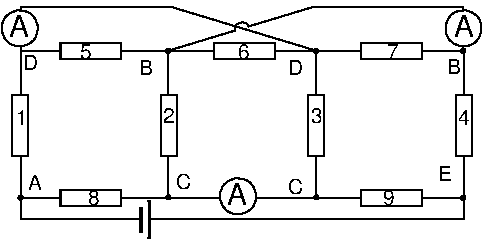
\includegraphics[width=\textwidth]{3ruutlah-a.pdf}\\
    \end{subfigure}
    \begin{subfigure}[h]{0.45\textwidth}
    \vspace{-10pt}
     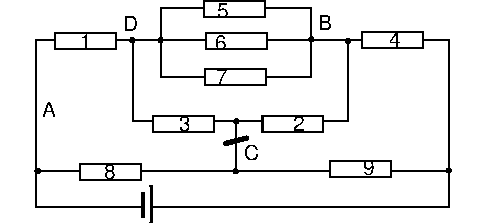
\includegraphics[width=\textwidth]{3ruutlah-b.pdf}
    \end{subfigure}
 \end{figure}

\newpage


\yl{KÄRBES} \punktid{12} Kui kärbes liigub mööda joonisel näidatud horisontaalset sirget, mis lõikub läätsega punktis A ja alustab liikumist väga kaugelt, siis kärbse kujutis liigub mööda kaldjoont, mis läbib punkti A ja fookust F (sest sirge kujutis on sirge ja need kaks sirget lõikuvad läätse tasandis) ning alustab liikumist punktist F eemaldudes alguses väga aeglaselt. Kujutise kiirus kasvab monotoonselt kuni jõuab lõpmatusse hetkel, mil kärbes läbib fokaaltasandi. Seega, kui kärbse kiirust kujutab horisontaalne vektor $v$ parempoolsel joonisel, siis kujutise kiiruse vektor erinevatel ajahetkedel on kujutatud kaldus olevate vektoritena $u$. On ilmne, et nende kahe vektori vahe $w$ on minimaalne siis, kui vektor $w$ on risti vektoriga $u$. Seega saame $u_{\min}=v\sin\alpha$. Kolmnurga $OAF$ põhjal $\sin\alpha=a/\sqrt{a^2+f^2}$ ning $u_{\min}=va/\sqrt{a^2+f^2}$.\\

\begin{center}
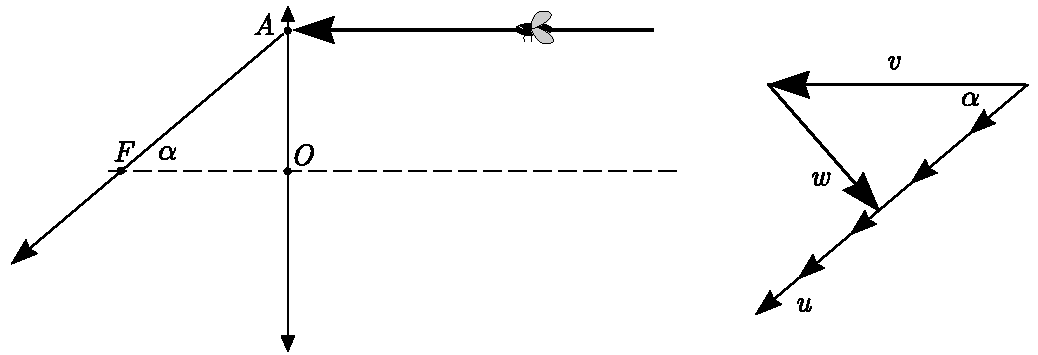
\includegraphics[scale=0.7]{kxrbes.pdf}
\end{center}

\yl{NIIT JA POOLSFÄÄR} \punktid{12} Et kera on maandatud, siis selle keskpunkti potentsiaal on 0. Superpositsiooniprintsiibi abil saame selle avaldada kui kera pinnale indutseeritud laengute $Q_i$ ja rõngal olevate laengute $q_j$ panuste summa: $0=\sum_i kQ_i/R+k\sum_jkq_j/l$, kus $l=\sqrt{r^2+d^2}$ on rõnga punktide kaugus kera keskpunktist. Summas saab konstandid sulgude ette tuua: $0=\frac kR \sum_iQ_i+\frac kl\sum_jq_j=kQ/R+kq/l$, seega $Q=-qR/\sqrt{r^2+d^2}$.

\yl{PÖÖRDUV ELEKTRIVÄLI} \punktid{12} Et osakese $x$-telje sihiline keskmine kiirus $v_x$ oleks null, peab ajaperioodidel $4nT+T\le t < 4nT+2T$ ja  $4nT+3T\le t < 4nT+4T$ olema $v_x$ väärtused võrdsed ja vastasmärgilised, vastavalt $u$ ja $-u$; ajavahemikul $4nT+2T\le t < 4nT+3T$ annab elektriväli osakesele $x$-suunalise impulsi $-E_0qT$, seetõttu
$$2mu=E_0qT \;\;\Rightarrow\;\; u=\frac{E_0qT}{2m}.$$
Järgneva veerandperioodi jooksul püsib osakese $x$-sihiline kiirus konstantselt võrdne $u$-ga ning seega nihkub osake sel ajal $x$-telje sihis $x_1=uT$ võrra. Järgneva kaheksandikperioodi jooksul (ketusega $T/2$) kahaneb kiirus lineaarselt ajas nullini, seetõttu on täiendav nihe leitav keskmise kiiruse $\frac u2$ abil, $x_2=\frac u2\cdot \frac T2=uT/4$; sümmeetria tõttu toimus samasugune nihe ka konstantse kiirusega veerandperioodile eelenenud kaheksandikperioodi jooksul, st kogunihe (ja seega trajektoori $x$-telje sihiline läbimõõt) on $$x_1+2x_2=\frac32 uT=\frac{3E_0qT^2}{4m}.$$
Sümmeetria tõttu on $y$-telje sihiline läbimõõt samasugune. Trajektooriks on kujund, mis koosneb neljast paraboolist --- iga järgmine parabool on saadud eelmisest täisnurga võrra pööramisel (paraboolide pikkused peavad olema sellised, et otspunktides oleks tõusnurk $45^\circ$: kõverad peavad liituma ilma murdepunktita.

\vspace{-20pt}
\begin{center}
  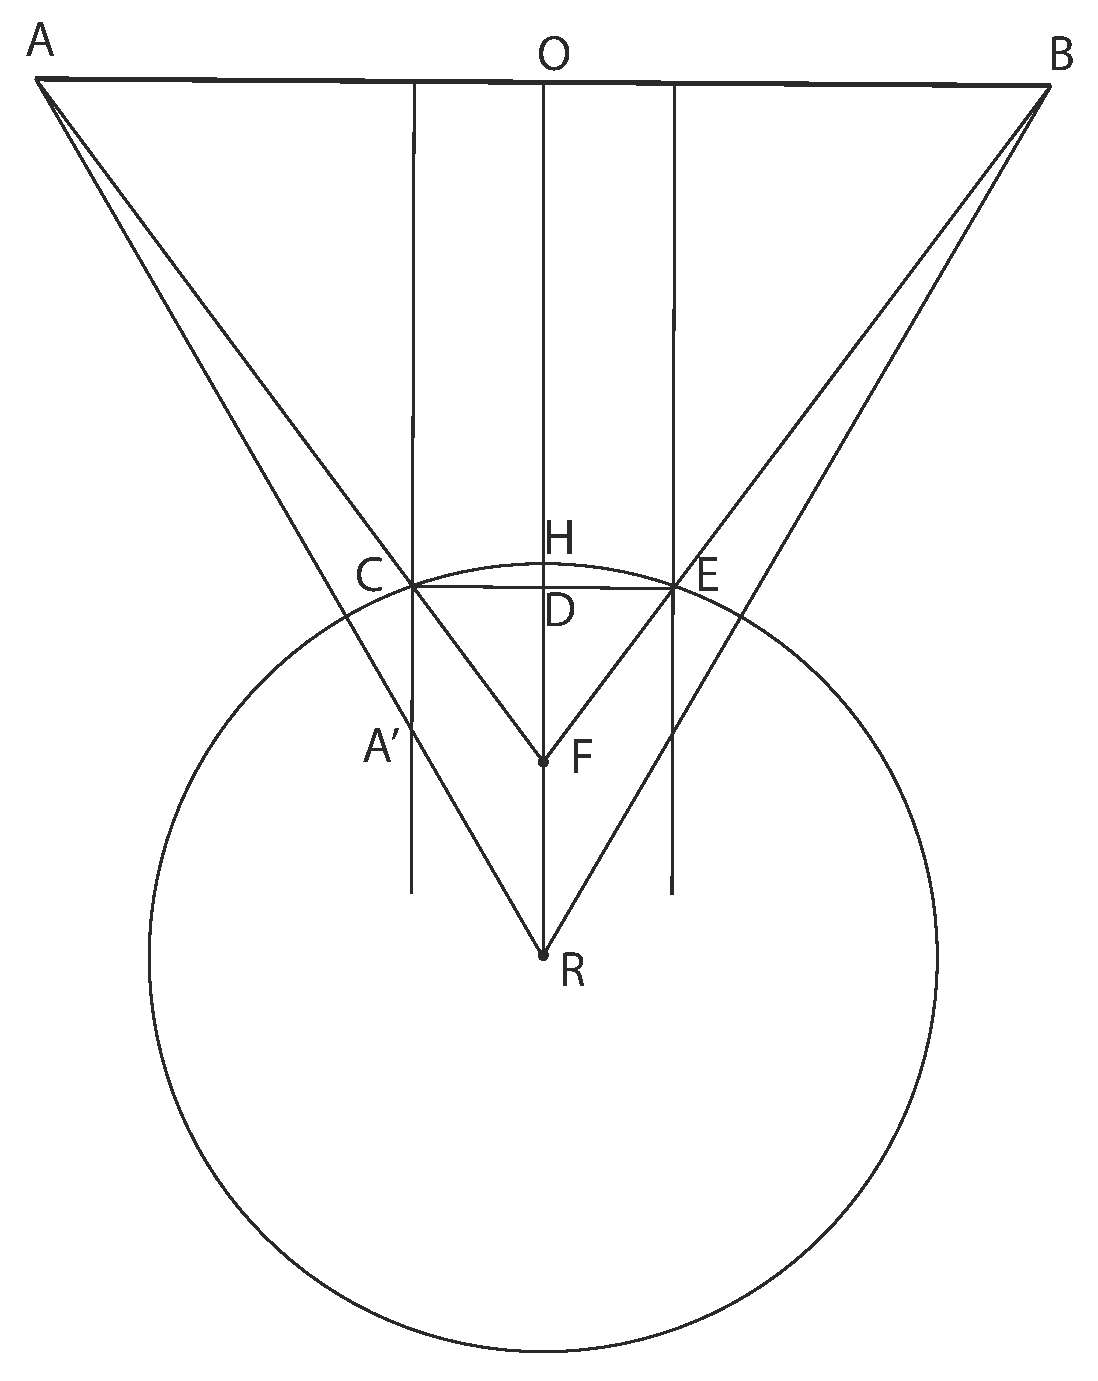
\includegraphics[width=0.6\textwidth]{kumerpeegellahendus}
\end{center}
\vspace{-20pt}


\end{document}

